% Created by tikzDevice version 0.12.6 on 2026-08-08 12:11:36
% !TEX encoding = UTF-8 Unicode
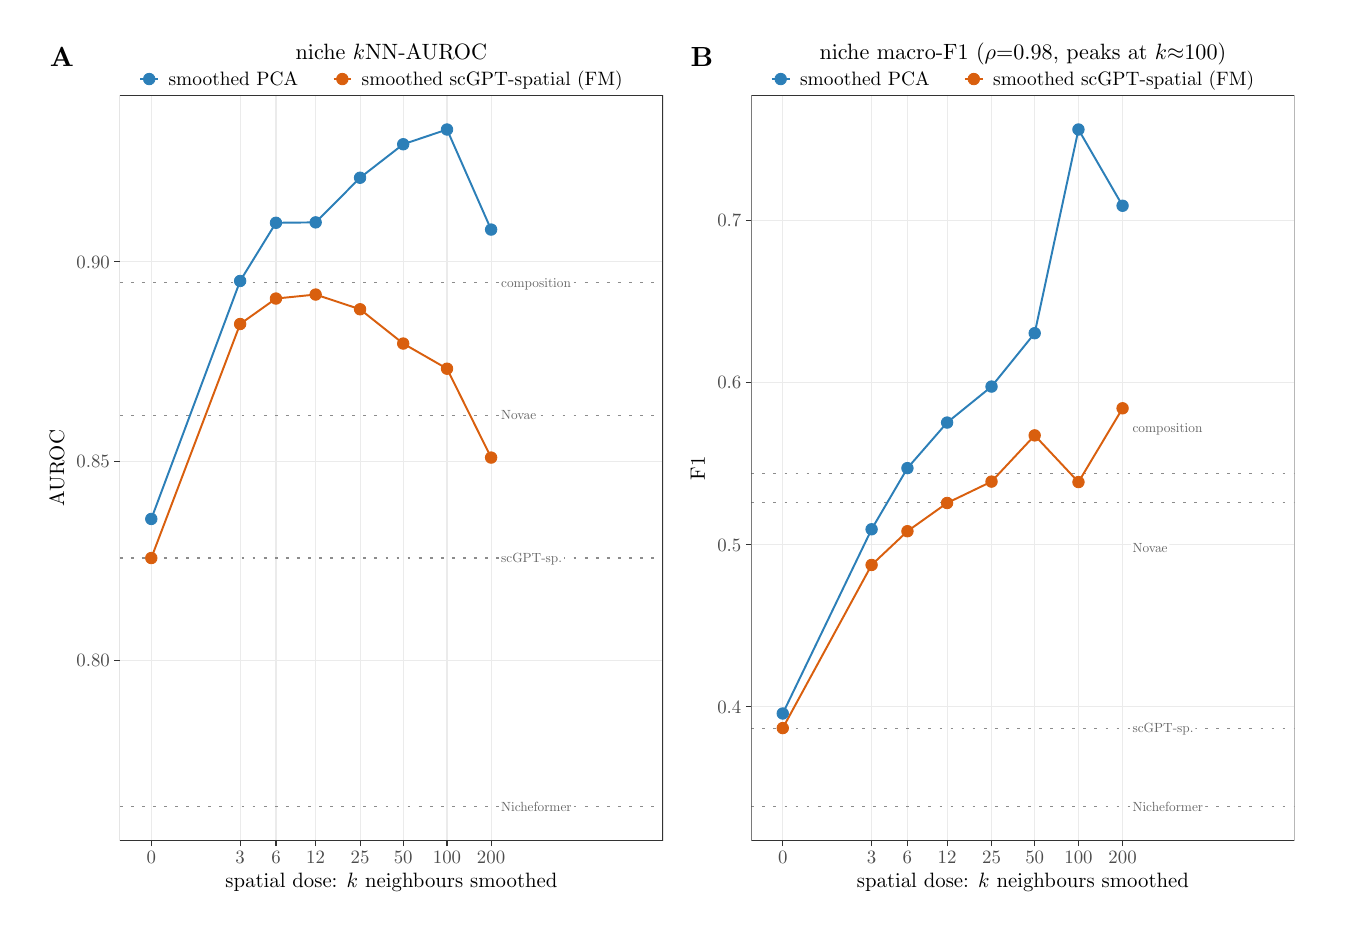
\begin{tikzpicture}[x=1pt,y=1pt]
\definecolor{fillColor}{RGB}{255,255,255}
\path[use as bounding box,fill=fillColor,fill opacity=0.00] (0,0) rectangle (469.75,317.99);
\begin{scope}
\path[clip] (  0.00,  0.00) rectangle (469.75,317.99);
\definecolor{drawColor}{RGB}{255,255,255}
\definecolor{fillColor}{RGB}{255,255,255}

\path[draw=drawColor,line width= 0.4pt,line join=round,line cap=round,fill=fillColor] ( -0.00,  0.00) rectangle (469.76,317.99);
\end{scope}
\begin{scope}
\path[clip] (  4.00,  3.00) rectangle (235.58,314.99);
\definecolor{drawColor}{RGB}{255,255,255}
\definecolor{fillColor}{RGB}{255,255,255}

\path[draw=drawColor,line width= 0.4pt,line join=round,line cap=round,fill=fillColor] (  4.00,  3.00) rectangle (235.58,314.99);
\end{scope}
\begin{scope}
\path[clip] (235.58,  3.00) rectangle (463.76,314.99);
\definecolor{drawColor}{RGB}{255,255,255}
\definecolor{fillColor}{RGB}{255,255,255}

\path[draw=drawColor,line width= 0.4pt,line join=round,line cap=round,fill=fillColor] (235.58,  3.00) rectangle (463.75,314.99);
\end{scope}
\begin{scope}
\path[clip] ( 33.31, 24.23) rectangle (229.58,293.42);
\definecolor{fillColor}{RGB}{255,255,255}

\path[fill=fillColor] ( 33.31, 24.23) rectangle (229.58,293.42);
\definecolor{drawColor}{gray}{0.92}

\path[draw=drawColor,line width= 0.4pt,line join=round] ( 33.31, 89.33) --
	(229.58, 89.33);

\path[draw=drawColor,line width= 0.4pt,line join=round] ( 33.31,161.35) --
	(229.58,161.35);

\path[draw=drawColor,line width= 0.4pt,line join=round] ( 33.31,233.37) --
	(229.58,233.37);

\path[draw=drawColor,line width= 0.4pt,line join=round] ( 44.67, 24.23) --
	( 44.67,293.42);

\path[draw=drawColor,line width= 0.4pt,line join=round] ( 76.77, 24.23) --
	( 76.77,293.42);

\path[draw=drawColor,line width= 0.4pt,line join=round] ( 89.72, 24.23) --
	( 89.72,293.42);

\path[draw=drawColor,line width= 0.4pt,line join=round] (104.06, 24.23) --
	(104.06,293.42);

\path[draw=drawColor,line width= 0.4pt,line join=round] (120.11, 24.23) --
	(120.11,293.42);

\path[draw=drawColor,line width= 0.4pt,line join=round] (135.70, 24.23) --
	(135.70,293.42);

\path[draw=drawColor,line width= 0.4pt,line join=round] (151.53, 24.23) --
	(151.53,293.42);

\path[draw=drawColor,line width= 0.4pt,line join=round] (167.46, 24.23) --
	(167.46,293.42);
\definecolor{drawColor}{gray}{0.55}

\path[draw=drawColor,line width= 0.4pt,dash pattern=on 1pt off 3pt ,line join=round] ( 33.31,177.91) -- (229.58,177.91);

\path[draw=drawColor,line width= 0.4pt,dash pattern=on 1pt off 3pt ,line join=round] ( 33.31,126.34) -- (229.58,126.34);

\path[draw=drawColor,line width= 0.4pt,dash pattern=on 1pt off 3pt ,line join=round] ( 33.31, 36.46) -- (229.58, 36.46);

\path[draw=drawColor,line width= 0.4pt,dash pattern=on 1pt off 3pt ,line join=round] ( 33.31,225.88) -- (229.58,225.88);

\path[fill=fillColor] (171.45,175.30) --
	(183.47,175.30) --
	(183.43,175.31) --
	(183.57,175.31) --
	(183.71,175.34) --
	(183.84,175.39) --
	(183.96,175.46) --
	(184.07,175.55) --
	(184.17,175.65) --
	(184.24,175.77) --
	(184.30,175.90) --
	(184.33,176.04) --
	(184.34,176.18) --
	(184.34,176.18) --
	(184.34,179.64) --
	(184.34,179.64) --
	(184.33,179.78) --
	(184.30,179.92) --
	(184.24,180.05) --
	(184.17,180.17) --
	(184.07,180.27) --
	(183.96,180.36) --
	(183.84,180.43) --
	(183.71,180.48) --
	(183.57,180.51) --
	(183.47,180.52) --
	(171.45,180.52) --
	(171.56,180.51) --
	(171.42,180.52) --
	(171.28,180.50) --
	(171.14,180.46) --
	(171.02,180.40) --
	(170.90,180.32) --
	(170.80,180.22) --
	(170.71,180.11) --
	(170.65,179.99) --
	(170.60,179.85) --
	(170.58,179.71) --
	(170.58,179.64) --
	(170.58,176.18) --
	(170.58,176.25) --
	(170.58,176.11) --
	(170.60,175.97) --
	(170.65,175.84) --
	(170.71,175.71) --
	(170.80,175.60) --
	(170.90,175.50) --
	(171.02,175.42) --
	(171.14,175.36) --
	(171.28,175.32) --
	(171.42,175.31) --
	cycle;
\end{scope}
\begin{scope}
\path[clip] ( 33.31, 24.23) rectangle (229.58,293.42);
\definecolor{drawColor}{gray}{0.40}

\node[text=drawColor,anchor=base west,inner sep=0pt, outer sep=0pt, scale=  0.48] at (171.08,176.25) {Novae};
\end{scope}
\begin{scope}
\path[clip] ( 33.31, 24.23) rectangle (229.58,293.42);
\definecolor{fillColor}{RGB}{255,255,255}

\path[fill=fillColor] (171.45,123.74) --
	(192.89,123.74) --
	(192.85,123.74) --
	(193.00,123.75) --
	(193.13,123.77) --
	(193.26,123.82) --
	(193.39,123.89) --
	(193.50,123.98) --
	(193.59,124.09) --
	(193.66,124.21) --
	(193.72,124.34) --
	(193.75,124.47) --
	(193.76,124.61) --
	(193.76,124.61) --
	(193.76,128.08) --
	(193.76,128.08) --
	(193.75,128.22) --
	(193.72,128.35) --
	(193.66,128.48) --
	(193.59,128.60) --
	(193.50,128.71) --
	(193.39,128.80) --
	(193.26,128.87) --
	(193.13,128.92) --
	(193.00,128.94) --
	(192.89,128.95) --
	(171.45,128.95) --
	(171.56,128.94) --
	(171.42,128.95) --
	(171.28,128.93) --
	(171.14,128.89) --
	(171.02,128.83) --
	(170.90,128.75) --
	(170.80,128.66) --
	(170.71,128.54) --
	(170.65,128.42) --
	(170.60,128.29) --
	(170.58,128.15) --
	(170.58,128.08) --
	(170.58,124.61) --
	(170.58,124.68) --
	(170.58,124.54) --
	(170.60,124.40) --
	(170.65,124.27) --
	(170.71,124.15) --
	(170.80,124.03) --
	(170.90,123.94) --
	(171.02,123.86) --
	(171.14,123.80) --
	(171.28,123.76) --
	(171.42,123.74) --
	cycle;
\end{scope}
\begin{scope}
\path[clip] ( 33.31, 24.23) rectangle (229.58,293.42);
\definecolor{drawColor}{gray}{0.40}

\node[text=drawColor,anchor=base west,inner sep=0pt, outer sep=0pt, scale=  0.48] at (171.08,124.68) {scGPT-sp.};
\end{scope}
\begin{scope}
\path[clip] ( 33.31, 24.23) rectangle (229.58,293.42);
\definecolor{fillColor}{RGB}{255,255,255}

\path[fill=fillColor] (171.45, 33.86) --
	(196.39, 33.86) --
	(196.35, 33.86) --
	(196.49, 33.87) --
	(196.63, 33.89) --
	(196.76, 33.94) --
	(196.89, 34.01) --
	(196.99, 34.10) --
	(197.09, 34.21) --
	(197.16, 34.33) --
	(197.22, 34.46) --
	(197.25, 34.59) --
	(197.26, 34.73) --
	(197.26, 34.73) --
	(197.26, 38.20) --
	(197.26, 38.20) --
	(197.25, 38.34) --
	(197.22, 38.47) --
	(197.16, 38.60) --
	(197.09, 38.72) --
	(196.99, 38.83) --
	(196.89, 38.92) --
	(196.76, 38.99) --
	(196.63, 39.04) --
	(196.49, 39.06) --
	(196.39, 39.07) --
	(171.45, 39.07) --
	(171.56, 39.06) --
	(171.42, 39.07) --
	(171.28, 39.05) --
	(171.14, 39.01) --
	(171.02, 38.95) --
	(170.90, 38.87) --
	(170.80, 38.78) --
	(170.71, 38.66) --
	(170.65, 38.54) --
	(170.60, 38.41) --
	(170.58, 38.27) --
	(170.58, 38.20) --
	(170.58, 34.73) --
	(170.58, 34.80) --
	(170.58, 34.66) --
	(170.60, 34.52) --
	(170.65, 34.39) --
	(170.71, 34.27) --
	(170.80, 34.15) --
	(170.90, 34.06) --
	(171.02, 33.98) --
	(171.14, 33.92) --
	(171.28, 33.88) --
	(171.42, 33.86) --
	cycle;
\end{scope}
\begin{scope}
\path[clip] ( 33.31, 24.23) rectangle (229.58,293.42);
\definecolor{drawColor}{gray}{0.40}

\node[text=drawColor,anchor=base west,inner sep=0pt, outer sep=0pt, scale=  0.48] at (171.08, 34.80) {Nicheformer};
\end{scope}
\begin{scope}
\path[clip] ( 33.31, 24.23) rectangle (229.58,293.42);
\definecolor{fillColor}{RGB}{255,255,255}

\path[fill=fillColor] (171.45,223.27) --
	(196.12,223.27) --
	(196.09,223.27) --
	(196.23,223.28) --
	(196.36,223.30) --
	(196.50,223.35) --
	(196.62,223.42) --
	(196.73,223.51) --
	(196.82,223.62) --
	(196.89,223.74) --
	(196.95,223.87) --
	(196.98,224.00) --
	(196.99,224.14) --
	(196.99,224.14) --
	(196.99,227.61) --
	(196.99,227.61) --
	(196.98,227.75) --
	(196.95,227.88) --
	(196.89,228.01) --
	(196.82,228.13) --
	(196.73,228.24) --
	(196.62,228.33) --
	(196.50,228.40) --
	(196.36,228.45) --
	(196.23,228.48) --
	(196.12,228.48) --
	(171.45,228.48) --
	(171.56,228.48) --
	(171.42,228.48) --
	(171.28,228.46) --
	(171.14,228.43) --
	(171.02,228.36) --
	(170.90,228.28) --
	(170.80,228.19) --
	(170.71,228.08) --
	(170.65,227.95) --
	(170.60,227.82) --
	(170.58,227.68) --
	(170.58,227.61) --
	(170.58,224.14) --
	(170.58,224.21) --
	(170.58,224.07) --
	(170.60,223.93) --
	(170.65,223.80) --
	(170.71,223.68) --
	(170.80,223.56) --
	(170.90,223.47) --
	(171.02,223.39) --
	(171.14,223.33) --
	(171.28,223.29) --
	(171.42,223.27) --
	cycle;
\end{scope}
\begin{scope}
\path[clip] ( 33.31, 24.23) rectangle (229.58,293.42);
\definecolor{drawColor}{gray}{0.40}

\node[text=drawColor,anchor=base west,inner sep=0pt, outer sep=0pt, scale=  0.48] at (171.08,224.21) {composition};
\end{scope}
\begin{scope}
\path[clip] ( 33.31, 24.23) rectangle (229.58,293.42);
\definecolor{drawColor}{RGB}{44,127,184}

\path[draw=drawColor,line width= 0.7pt,line join=round] ( 44.67,140.46) --
	( 76.77,226.45) --
	( 89.72,247.48) --
	(104.06,247.63) --
	(120.11,263.76) --
	(135.70,275.86) --
	(151.53,281.19) --
	(167.46,245.03);
\definecolor{drawColor}{RGB}{217,95,14}

\path[draw=drawColor,line width= 0.7pt,line join=round] ( 44.67,126.34) --
	( 76.77,210.90) --
	( 89.72,220.11) --
	(104.06,221.55) --
	(120.11,216.23) --
	(135.70,203.84) --
	(151.53,194.76) --
	(167.46,162.64);
\definecolor{drawColor}{RGB}{44,127,184}
\definecolor{fillColor}{RGB}{44,127,184}

\path[draw=drawColor,line width= 0.3pt,line join=round,line cap=round,fill=fillColor] ( 44.67,140.46) circle (  2.08);

\path[draw=drawColor,line width= 0.3pt,line join=round,line cap=round,fill=fillColor] ( 76.77,226.45) circle (  2.08);

\path[draw=drawColor,line width= 0.3pt,line join=round,line cap=round,fill=fillColor] ( 89.72,247.48) circle (  2.08);

\path[draw=drawColor,line width= 0.3pt,line join=round,line cap=round,fill=fillColor] (104.06,247.63) circle (  2.08);

\path[draw=drawColor,line width= 0.3pt,line join=round,line cap=round,fill=fillColor] (120.11,263.76) circle (  2.08);

\path[draw=drawColor,line width= 0.3pt,line join=round,line cap=round,fill=fillColor] (135.70,275.86) circle (  2.08);

\path[draw=drawColor,line width= 0.3pt,line join=round,line cap=round,fill=fillColor] (151.53,281.19) circle (  2.08);

\path[draw=drawColor,line width= 0.3pt,line join=round,line cap=round,fill=fillColor] (167.46,245.03) circle (  2.08);
\definecolor{drawColor}{RGB}{217,95,14}
\definecolor{fillColor}{RGB}{217,95,14}

\path[draw=drawColor,line width= 0.3pt,line join=round,line cap=round,fill=fillColor] ( 44.67,126.34) circle (  2.08);

\path[draw=drawColor,line width= 0.3pt,line join=round,line cap=round,fill=fillColor] ( 76.77,210.90) circle (  2.08);

\path[draw=drawColor,line width= 0.3pt,line join=round,line cap=round,fill=fillColor] ( 89.72,220.11) circle (  2.08);

\path[draw=drawColor,line width= 0.3pt,line join=round,line cap=round,fill=fillColor] (104.06,221.55) circle (  2.08);

\path[draw=drawColor,line width= 0.3pt,line join=round,line cap=round,fill=fillColor] (120.11,216.23) circle (  2.08);

\path[draw=drawColor,line width= 0.3pt,line join=round,line cap=round,fill=fillColor] (135.70,203.84) circle (  2.08);

\path[draw=drawColor,line width= 0.3pt,line join=round,line cap=round,fill=fillColor] (151.53,194.76) circle (  2.08);

\path[draw=drawColor,line width= 0.3pt,line join=round,line cap=round,fill=fillColor] (167.46,162.64) circle (  2.08);
\definecolor{drawColor}{gray}{0.20}

\path[draw=drawColor,line width= 0.4pt,line join=round,line cap=round] ( 33.31, 24.23) rectangle (229.58,293.42);
\end{scope}
\begin{scope}
\path[clip] (  0.00,  0.00) rectangle (469.75,317.99);
\definecolor{drawColor}{gray}{0.30}

\node[text=drawColor,anchor=base east,inner sep=0pt, outer sep=0pt, scale=  0.68] at ( 29.71, 86.99) {0.80};

\node[text=drawColor,anchor=base east,inner sep=0pt, outer sep=0pt, scale=  0.68] at ( 29.71,159.00) {0.85};

\node[text=drawColor,anchor=base east,inner sep=0pt, outer sep=0pt, scale=  0.68] at ( 29.71,231.02) {0.90};
\end{scope}
\begin{scope}
\path[clip] (  0.00,  0.00) rectangle (469.75,317.99);
\definecolor{drawColor}{gray}{0.20}

\path[draw=drawColor,line width= 0.4pt,line join=round] ( 31.31, 89.33) --
	( 33.31, 89.33);

\path[draw=drawColor,line width= 0.4pt,line join=round] ( 31.31,161.35) --
	( 33.31,161.35);

\path[draw=drawColor,line width= 0.4pt,line join=round] ( 31.31,233.37) --
	( 33.31,233.37);
\end{scope}
\begin{scope}
\path[clip] (  0.00,  0.00) rectangle (469.75,317.99);
\definecolor{drawColor}{gray}{0.20}

\path[draw=drawColor,line width= 0.4pt,line join=round] ( 44.67, 22.23) --
	( 44.67, 24.23);

\path[draw=drawColor,line width= 0.4pt,line join=round] ( 76.77, 22.23) --
	( 76.77, 24.23);

\path[draw=drawColor,line width= 0.4pt,line join=round] ( 89.72, 22.23) --
	( 89.72, 24.23);

\path[draw=drawColor,line width= 0.4pt,line join=round] (104.06, 22.23) --
	(104.06, 24.23);

\path[draw=drawColor,line width= 0.4pt,line join=round] (120.11, 22.23) --
	(120.11, 24.23);

\path[draw=drawColor,line width= 0.4pt,line join=round] (135.70, 22.23) --
	(135.70, 24.23);

\path[draw=drawColor,line width= 0.4pt,line join=round] (151.53, 22.23) --
	(151.53, 24.23);

\path[draw=drawColor,line width= 0.4pt,line join=round] (167.46, 22.23) --
	(167.46, 24.23);
\end{scope}
\begin{scope}
\path[clip] (  0.00,  0.00) rectangle (469.75,317.99);
\definecolor{drawColor}{gray}{0.30}

\node[text=drawColor,anchor=base,inner sep=0pt, outer sep=0pt, scale=  0.68] at ( 44.67, 15.95) {0};

\node[text=drawColor,anchor=base,inner sep=0pt, outer sep=0pt, scale=  0.68] at ( 76.77, 15.95) {3};

\node[text=drawColor,anchor=base,inner sep=0pt, outer sep=0pt, scale=  0.68] at ( 89.72, 15.95) {6};

\node[text=drawColor,anchor=base,inner sep=0pt, outer sep=0pt, scale=  0.68] at (104.06, 15.95) {12};

\node[text=drawColor,anchor=base,inner sep=0pt, outer sep=0pt, scale=  0.68] at (120.11, 15.95) {25};

\node[text=drawColor,anchor=base,inner sep=0pt, outer sep=0pt, scale=  0.68] at (135.70, 15.95) {50};

\node[text=drawColor,anchor=base,inner sep=0pt, outer sep=0pt, scale=  0.68] at (151.53, 15.95) {100};

\node[text=drawColor,anchor=base,inner sep=0pt, outer sep=0pt, scale=  0.68] at (167.46, 15.95) {200};
\end{scope}
\begin{scope}
\path[clip] (  0.00,  0.00) rectangle (469.75,317.99);
\definecolor{drawColor}{RGB}{0,0,0}

\node[text=drawColor,anchor=base,inner sep=0pt, outer sep=0pt, scale=  0.75] at (131.44,  7.46) {spatial dose: $k$ neighbours smoothed};
\end{scope}
\begin{scope}
\path[clip] (  0.00,  0.00) rectangle (469.75,317.99);
\definecolor{drawColor}{RGB}{0,0,0}

\node[text=drawColor,rotate= 90.00,anchor=base,inner sep=0pt, outer sep=0pt, scale=  0.75] at ( 13.17,158.83) {AUROC};
\end{scope}
\begin{scope}
\path[clip] (  0.00,  0.00) rectangle (469.75,317.99);
\definecolor{fillColor}{RGB}{255,255,255}

\path[fill=fillColor] ( 38.92,295.42) rectangle (223.97,303.42);
\end{scope}
\begin{scope}
\path[clip] (  0.00,  0.00) rectangle (469.75,317.99);
\definecolor{fillColor}{RGB}{255,255,255}

\path[fill=fillColor] ( 39.92,295.42) rectangle ( 47.92,303.42);
\definecolor{drawColor}{RGB}{44,127,184}

\path[draw=drawColor,line width= 0.7pt,line join=round] ( 40.72,299.42) -- ( 47.12,299.42);
\definecolor{fillColor}{RGB}{44,127,184}

\path[draw=drawColor,line width= 0.3pt,line join=round,line cap=round,fill=fillColor] ( 43.92,299.42) circle (  2.08);
\end{scope}
\begin{scope}
\path[clip] (  0.00,  0.00) rectangle (469.75,317.99);
\definecolor{fillColor}{RGB}{255,255,255}

\path[fill=fillColor] (109.71,295.42) rectangle (117.71,303.42);
\definecolor{drawColor}{RGB}{217,95,14}

\path[draw=drawColor,line width= 0.7pt,line join=round] (110.51,299.42) -- (116.91,299.42);
\definecolor{fillColor}{RGB}{217,95,14}

\path[draw=drawColor,line width= 0.3pt,line join=round,line cap=round,fill=fillColor] (113.71,299.42) circle (  2.08);
\end{scope}
\begin{scope}
\path[clip] (  0.00,  0.00) rectangle (469.75,317.99);
\definecolor{drawColor}{RGB}{0,0,0}

\node[text=drawColor,anchor=base west,inner sep=0pt, outer sep=0pt, scale=  0.70] at ( 50.92,297.01) {smoothed PCA};
\end{scope}
\begin{scope}
\path[clip] (  0.00,  0.00) rectangle (469.75,317.99);
\definecolor{drawColor}{RGB}{0,0,0}

\node[text=drawColor,anchor=base west,inner sep=0pt, outer sep=0pt, scale=  0.70] at (120.71,297.01) {smoothed scGPT-spatial (FM)};
\end{scope}
\begin{scope}
\path[clip] (  0.00,  0.00) rectangle (469.75,317.99);
\definecolor{drawColor}{RGB}{0,0,0}

\node[text=drawColor,anchor=base,inner sep=0pt, outer sep=0pt, scale=  0.80] at (131.44,306.48) {niche $k$NN-AUROC};
\end{scope}
\begin{scope}
\path[clip] (  0.00,  0.00) rectangle (469.75,317.99);
\definecolor{drawColor}{RGB}{0,0,0}

\node[text=drawColor,anchor=base,inner sep=0pt, outer sep=0pt, scale=  1.00] at ( 12.35,304.11) {\bfseries A};
\end{scope}
\begin{scope}
\path[clip] (261.49, 24.23) rectangle (457.75,293.42);
\definecolor{fillColor}{RGB}{255,255,255}

\path[fill=fillColor] (261.49, 24.23) rectangle (457.75,293.42);
\definecolor{drawColor}{gray}{0.92}

\path[draw=drawColor,line width= 0.4pt,line join=round] (261.49, 72.62) --
	(457.75, 72.62);

\path[draw=drawColor,line width= 0.4pt,line join=round] (261.49,131.22) --
	(457.75,131.22);

\path[draw=drawColor,line width= 0.4pt,line join=round] (261.49,189.83) --
	(457.75,189.83);

\path[draw=drawColor,line width= 0.4pt,line join=round] (261.49,248.43) --
	(457.75,248.43);

\path[draw=drawColor,line width= 0.4pt,line join=round] (272.85, 24.23) --
	(272.85,293.42);

\path[draw=drawColor,line width= 0.4pt,line join=round] (304.95, 24.23) --
	(304.95,293.42);

\path[draw=drawColor,line width= 0.4pt,line join=round] (317.90, 24.23) --
	(317.90,293.42);

\path[draw=drawColor,line width= 0.4pt,line join=round] (332.23, 24.23) --
	(332.23,293.42);

\path[draw=drawColor,line width= 0.4pt,line join=round] (348.28, 24.23) --
	(348.28,293.42);

\path[draw=drawColor,line width= 0.4pt,line join=round] (363.88, 24.23) --
	(363.88,293.42);

\path[draw=drawColor,line width= 0.4pt,line join=round] (379.70, 24.23) --
	(379.70,293.42);

\path[draw=drawColor,line width= 0.4pt,line join=round] (395.64, 24.23) --
	(395.64,293.42);
\definecolor{drawColor}{gray}{0.55}

\path[draw=drawColor,line width= 0.4pt,dash pattern=on 1pt off 3pt ,line join=round] (261.49,146.28) -- (457.75,146.28);

\path[draw=drawColor,line width= 0.4pt,dash pattern=on 1pt off 3pt ,line join=round] (261.49, 64.89) -- (457.75, 64.89);

\path[draw=drawColor,line width= 0.4pt,dash pattern=on 1pt off 3pt ,line join=round] (261.49, 36.46) -- (457.75, 36.46);

\path[draw=drawColor,line width= 0.4pt,dash pattern=on 1pt off 3pt ,line join=round] (261.49,156.95) -- (457.75,156.95);

\path[fill=fillColor] (399.63,127.27) --
	(411.64,127.27) --
	(411.61,127.27) --
	(411.75,127.28) --
	(411.89,127.30) --
	(412.02,127.35) --
	(412.14,127.43) --
	(412.25,127.51) --
	(412.34,127.62) --
	(412.42,127.74) --
	(412.47,127.87) --
	(412.51,128.00) --
	(412.52,128.14) --
	(412.52,128.14) --
	(412.52,131.61) --
	(412.52,131.61) --
	(412.51,131.75) --
	(412.47,131.89) --
	(412.42,132.01) --
	(412.34,132.13) --
	(412.25,132.24) --
	(412.14,132.33) --
	(412.02,132.40) --
	(411.89,132.45) --
	(411.75,132.48) --
	(411.64,132.48) --
	(399.63,132.48) --
	(399.74,132.48) --
	(399.60,132.48) --
	(399.46,132.46) --
	(399.32,132.43) --
	(399.19,132.37) --
	(399.08,132.29) --
	(398.98,132.19) --
	(398.89,132.08) --
	(398.83,131.95) --
	(398.78,131.82) --
	(398.76,131.68) --
	(398.76,131.61) --
	(398.76,128.14) --
	(398.76,128.21) --
	(398.76,128.07) --
	(398.78,127.94) --
	(398.83,127.80) --
	(398.89,127.68) --
	(398.98,127.56) --
	(399.08,127.47) --
	(399.19,127.39) --
	(399.32,127.33) --
	(399.46,127.29) --
	(399.60,127.27) --
	cycle;
\end{scope}
\begin{scope}
\path[clip] (261.49, 24.23) rectangle (457.75,293.42);
\definecolor{drawColor}{gray}{0.40}

\node[text=drawColor,anchor=base west,inner sep=0pt, outer sep=0pt, scale=  0.48] at (399.26,128.21) {Novae};
\end{scope}
\begin{scope}
\path[clip] (261.49, 24.23) rectangle (457.75,293.42);
\definecolor{fillColor}{RGB}{255,255,255}

\path[fill=fillColor] (399.63, 62.28) --
	(421.07, 62.28) --
	(421.03, 62.28) --
	(421.17, 62.29) --
	(421.31, 62.32) --
	(421.44, 62.37) --
	(421.56, 62.44) --
	(421.67, 62.52) --
	(421.77, 62.63) --
	(421.84, 62.75) --
	(421.90, 62.88) --
	(421.93, 63.01) --
	(421.94, 63.15) --
	(421.94, 63.15) --
	(421.94, 66.62) --
	(421.94, 66.62) --
	(421.93, 66.76) --
	(421.90, 66.90) --
	(421.84, 67.02) --
	(421.77, 67.14) --
	(421.67, 67.25) --
	(421.56, 67.34) --
	(421.44, 67.41) --
	(421.31, 67.46) --
	(421.17, 67.49) --
	(421.07, 67.49) --
	(399.63, 67.49) --
	(399.74, 67.49) --
	(399.60, 67.49) --
	(399.46, 67.47) --
	(399.32, 67.44) --
	(399.19, 67.38) --
	(399.08, 67.30) --
	(398.98, 67.20) --
	(398.89, 67.09) --
	(398.83, 66.96) --
	(398.78, 66.83) --
	(398.76, 66.69) --
	(398.76, 66.62) --
	(398.76, 63.15) --
	(398.76, 63.22) --
	(398.76, 63.08) --
	(398.78, 62.95) --
	(398.83, 62.81) --
	(398.89, 62.69) --
	(398.98, 62.58) --
	(399.08, 62.48) --
	(399.19, 62.40) --
	(399.32, 62.34) --
	(399.46, 62.30) --
	(399.60, 62.28) --
	cycle;
\end{scope}
\begin{scope}
\path[clip] (261.49, 24.23) rectangle (457.75,293.42);
\definecolor{drawColor}{gray}{0.40}

\node[text=drawColor,anchor=base west,inner sep=0pt, outer sep=0pt, scale=  0.48] at (399.26, 63.22) {scGPT-sp.};
\end{scope}
\begin{scope}
\path[clip] (261.49, 24.23) rectangle (457.75,293.42);
\definecolor{fillColor}{RGB}{255,255,255}

\path[fill=fillColor] (399.63, 33.86) --
	(424.57, 33.86) --
	(424.53, 33.86) --
	(424.67, 33.87) --
	(424.81, 33.89) --
	(424.94, 33.94) --
	(425.06, 34.01) --
	(425.17, 34.10) --
	(425.27, 34.21) --
	(425.34, 34.33) --
	(425.40, 34.46) --
	(425.43, 34.59) --
	(425.44, 34.73) --
	(425.44, 34.73) --
	(425.44, 38.20) --
	(425.44, 38.20) --
	(425.43, 38.34) --
	(425.40, 38.47) --
	(425.34, 38.60) --
	(425.27, 38.72) --
	(425.17, 38.83) --
	(425.06, 38.92) --
	(424.94, 38.99) --
	(424.81, 39.04) --
	(424.67, 39.06) --
	(424.57, 39.07) --
	(399.63, 39.07) --
	(399.74, 39.06) --
	(399.60, 39.07) --
	(399.46, 39.05) --
	(399.32, 39.01) --
	(399.19, 38.95) --
	(399.08, 38.87) --
	(398.98, 38.78) --
	(398.89, 38.66) --
	(398.83, 38.54) --
	(398.78, 38.41) --
	(398.76, 38.27) --
	(398.76, 38.20) --
	(398.76, 34.73) --
	(398.76, 34.80) --
	(398.76, 34.66) --
	(398.78, 34.52) --
	(398.83, 34.39) --
	(398.89, 34.27) --
	(398.98, 34.15) --
	(399.08, 34.06) --
	(399.19, 33.98) --
	(399.32, 33.92) --
	(399.46, 33.88) --
	(399.60, 33.86) --
	cycle;
\end{scope}
\begin{scope}
\path[clip] (261.49, 24.23) rectangle (457.75,293.42);
\definecolor{drawColor}{gray}{0.40}

\node[text=drawColor,anchor=base west,inner sep=0pt, outer sep=0pt, scale=  0.48] at (399.26, 34.80) {Nicheformer};
\end{scope}
\begin{scope}
\path[clip] (261.49, 24.23) rectangle (457.75,293.42);
\definecolor{fillColor}{RGB}{255,255,255}

\path[fill=fillColor] (399.63,170.75) --
	(424.30,170.75) --
	(424.26,170.75) --
	(424.40,170.76) --
	(424.54,170.79) --
	(424.67,170.84) --
	(424.79,170.91) --
	(424.90,171.00) --
	(425.00,171.10) --
	(425.07,171.22) --
	(425.13,171.35) --
	(425.16,171.49) --
	(425.17,171.63) --
	(425.17,171.63) --
	(425.17,175.09) --
	(425.17,175.09) --
	(425.16,175.23) --
	(425.13,175.37) --
	(425.07,175.50) --
	(425.00,175.62) --
	(424.90,175.72) --
	(424.79,175.81) --
	(424.67,175.88) --
	(424.54,175.93) --
	(424.40,175.96) --
	(424.30,175.97) --
	(399.63,175.97) --
	(399.74,175.96) --
	(399.60,175.96) --
	(399.46,175.95) --
	(399.32,175.91) --
	(399.19,175.85) --
	(399.08,175.77) --
	(398.98,175.67) --
	(398.89,175.56) --
	(398.83,175.43) --
	(398.78,175.30) --
	(398.76,175.16) --
	(398.76,175.09) --
	(398.76,171.63) --
	(398.76,171.70) --
	(398.76,171.56) --
	(398.78,171.42) --
	(398.83,171.28) --
	(398.89,171.16) --
	(398.98,171.05) --
	(399.08,170.95) --
	(399.19,170.87) --
	(399.32,170.81) --
	(399.46,170.77) --
	(399.60,170.75) --
	cycle;
\end{scope}
\begin{scope}
\path[clip] (261.49, 24.23) rectangle (457.75,293.42);
\definecolor{drawColor}{gray}{0.40}

\node[text=drawColor,anchor=base west,inner sep=0pt, outer sep=0pt, scale=  0.48] at (399.26,171.69) {composition};
\end{scope}
\begin{scope}
\path[clip] (261.49, 24.23) rectangle (457.75,293.42);
\definecolor{drawColor}{RGB}{44,127,184}

\path[draw=drawColor,line width= 0.7pt,line join=round] (272.85, 70.16) --
	(304.95,136.73) --
	(317.90,158.83) --
	(332.23,175.29) --
	(348.28,188.30) --
	(363.88,207.58) --
	(379.70,281.19) --
	(395.64,253.64);
\definecolor{drawColor}{RGB}{217,95,14}

\path[draw=drawColor,line width= 0.7pt,line join=round] (272.85, 64.89) --
	(304.95,123.84) --
	(317.90,136.03) --
	(332.23,146.23) --
	(348.28,153.96) --
	(363.88,170.66) --
	(379.70,153.79) --
	(395.64,180.45);
\definecolor{drawColor}{RGB}{44,127,184}
\definecolor{fillColor}{RGB}{44,127,184}

\path[draw=drawColor,line width= 0.3pt,line join=round,line cap=round,fill=fillColor] (272.85, 70.16) circle (  2.08);

\path[draw=drawColor,line width= 0.3pt,line join=round,line cap=round,fill=fillColor] (304.95,136.73) circle (  2.08);

\path[draw=drawColor,line width= 0.3pt,line join=round,line cap=round,fill=fillColor] (317.90,158.83) circle (  2.08);

\path[draw=drawColor,line width= 0.3pt,line join=round,line cap=round,fill=fillColor] (332.23,175.29) circle (  2.08);

\path[draw=drawColor,line width= 0.3pt,line join=round,line cap=round,fill=fillColor] (348.28,188.30) circle (  2.08);

\path[draw=drawColor,line width= 0.3pt,line join=round,line cap=round,fill=fillColor] (363.88,207.58) circle (  2.08);

\path[draw=drawColor,line width= 0.3pt,line join=round,line cap=round,fill=fillColor] (379.70,281.19) circle (  2.08);

\path[draw=drawColor,line width= 0.3pt,line join=round,line cap=round,fill=fillColor] (395.64,253.64) circle (  2.08);
\definecolor{drawColor}{RGB}{217,95,14}
\definecolor{fillColor}{RGB}{217,95,14}

\path[draw=drawColor,line width= 0.3pt,line join=round,line cap=round,fill=fillColor] (272.85, 64.89) circle (  2.08);

\path[draw=drawColor,line width= 0.3pt,line join=round,line cap=round,fill=fillColor] (304.95,123.84) circle (  2.08);

\path[draw=drawColor,line width= 0.3pt,line join=round,line cap=round,fill=fillColor] (317.90,136.03) circle (  2.08);

\path[draw=drawColor,line width= 0.3pt,line join=round,line cap=round,fill=fillColor] (332.23,146.23) circle (  2.08);

\path[draw=drawColor,line width= 0.3pt,line join=round,line cap=round,fill=fillColor] (348.28,153.96) circle (  2.08);

\path[draw=drawColor,line width= 0.3pt,line join=round,line cap=round,fill=fillColor] (363.88,170.66) circle (  2.08);

\path[draw=drawColor,line width= 0.3pt,line join=round,line cap=round,fill=fillColor] (379.70,153.79) circle (  2.08);

\path[draw=drawColor,line width= 0.3pt,line join=round,line cap=round,fill=fillColor] (395.64,180.45) circle (  2.08);
\definecolor{drawColor}{gray}{0.20}

\path[draw=drawColor,line width= 0.4pt,line join=round,line cap=round] (261.49, 24.23) rectangle (457.75,293.42);
\end{scope}
\begin{scope}
\path[clip] (  0.00,  0.00) rectangle (469.75,317.99);
\definecolor{drawColor}{gray}{0.30}

\node[text=drawColor,anchor=base east,inner sep=0pt, outer sep=0pt, scale=  0.68] at (257.89, 70.28) {0.4};

\node[text=drawColor,anchor=base east,inner sep=0pt, outer sep=0pt, scale=  0.68] at (257.89,128.88) {0.5};

\node[text=drawColor,anchor=base east,inner sep=0pt, outer sep=0pt, scale=  0.68] at (257.89,187.48) {0.6};

\node[text=drawColor,anchor=base east,inner sep=0pt, outer sep=0pt, scale=  0.68] at (257.89,246.09) {0.7};
\end{scope}
\begin{scope}
\path[clip] (  0.00,  0.00) rectangle (469.75,317.99);
\definecolor{drawColor}{gray}{0.20}

\path[draw=drawColor,line width= 0.4pt,line join=round] (259.49, 72.62) --
	(261.49, 72.62);

\path[draw=drawColor,line width= 0.4pt,line join=round] (259.49,131.22) --
	(261.49,131.22);

\path[draw=drawColor,line width= 0.4pt,line join=round] (259.49,189.83) --
	(261.49,189.83);

\path[draw=drawColor,line width= 0.4pt,line join=round] (259.49,248.43) --
	(261.49,248.43);
\end{scope}
\begin{scope}
\path[clip] (  0.00,  0.00) rectangle (469.75,317.99);
\definecolor{drawColor}{gray}{0.20}

\path[draw=drawColor,line width= 0.4pt,line join=round] (272.85, 22.23) --
	(272.85, 24.23);

\path[draw=drawColor,line width= 0.4pt,line join=round] (304.95, 22.23) --
	(304.95, 24.23);

\path[draw=drawColor,line width= 0.4pt,line join=round] (317.90, 22.23) --
	(317.90, 24.23);

\path[draw=drawColor,line width= 0.4pt,line join=round] (332.23, 22.23) --
	(332.23, 24.23);

\path[draw=drawColor,line width= 0.4pt,line join=round] (348.28, 22.23) --
	(348.28, 24.23);

\path[draw=drawColor,line width= 0.4pt,line join=round] (363.88, 22.23) --
	(363.88, 24.23);

\path[draw=drawColor,line width= 0.4pt,line join=round] (379.70, 22.23) --
	(379.70, 24.23);

\path[draw=drawColor,line width= 0.4pt,line join=round] (395.64, 22.23) --
	(395.64, 24.23);
\end{scope}
\begin{scope}
\path[clip] (  0.00,  0.00) rectangle (469.75,317.99);
\definecolor{drawColor}{gray}{0.30}

\node[text=drawColor,anchor=base,inner sep=0pt, outer sep=0pt, scale=  0.68] at (272.85, 15.95) {0};

\node[text=drawColor,anchor=base,inner sep=0pt, outer sep=0pt, scale=  0.68] at (304.95, 15.95) {3};

\node[text=drawColor,anchor=base,inner sep=0pt, outer sep=0pt, scale=  0.68] at (317.90, 15.95) {6};

\node[text=drawColor,anchor=base,inner sep=0pt, outer sep=0pt, scale=  0.68] at (332.23, 15.95) {12};

\node[text=drawColor,anchor=base,inner sep=0pt, outer sep=0pt, scale=  0.68] at (348.28, 15.95) {25};

\node[text=drawColor,anchor=base,inner sep=0pt, outer sep=0pt, scale=  0.68] at (363.88, 15.95) {50};

\node[text=drawColor,anchor=base,inner sep=0pt, outer sep=0pt, scale=  0.68] at (379.70, 15.95) {100};

\node[text=drawColor,anchor=base,inner sep=0pt, outer sep=0pt, scale=  0.68] at (395.64, 15.95) {200};
\end{scope}
\begin{scope}
\path[clip] (  0.00,  0.00) rectangle (469.75,317.99);
\definecolor{drawColor}{RGB}{0,0,0}

\node[text=drawColor,anchor=base,inner sep=0pt, outer sep=0pt, scale=  0.75] at (359.62,  7.46) {spatial dose: $k$ neighbours smoothed};
\end{scope}
\begin{scope}
\path[clip] (  0.00,  0.00) rectangle (469.75,317.99);
\definecolor{drawColor}{RGB}{0,0,0}

\node[text=drawColor,rotate= 90.00,anchor=base,inner sep=0pt, outer sep=0pt, scale=  0.75] at (244.74,158.83) {F1};
\end{scope}
\begin{scope}
\path[clip] (  0.00,  0.00) rectangle (469.75,317.99);
\definecolor{fillColor}{RGB}{255,255,255}

\path[fill=fillColor] (267.10,295.42) rectangle (452.14,303.42);
\end{scope}
\begin{scope}
\path[clip] (  0.00,  0.00) rectangle (469.75,317.99);
\definecolor{fillColor}{RGB}{255,255,255}

\path[fill=fillColor] (268.10,295.42) rectangle (276.10,303.42);
\definecolor{drawColor}{RGB}{44,127,184}

\path[draw=drawColor,line width= 0.7pt,line join=round] (268.90,299.42) -- (275.30,299.42);
\definecolor{fillColor}{RGB}{44,127,184}

\path[draw=drawColor,line width= 0.3pt,line join=round,line cap=round,fill=fillColor] (272.10,299.42) circle (  2.08);
\end{scope}
\begin{scope}
\path[clip] (  0.00,  0.00) rectangle (469.75,317.99);
\definecolor{fillColor}{RGB}{255,255,255}

\path[fill=fillColor] (337.89,295.42) rectangle (345.89,303.42);
\definecolor{drawColor}{RGB}{217,95,14}

\path[draw=drawColor,line width= 0.7pt,line join=round] (338.69,299.42) -- (345.09,299.42);
\definecolor{fillColor}{RGB}{217,95,14}

\path[draw=drawColor,line width= 0.3pt,line join=round,line cap=round,fill=fillColor] (341.89,299.42) circle (  2.08);
\end{scope}
\begin{scope}
\path[clip] (  0.00,  0.00) rectangle (469.75,317.99);
\definecolor{drawColor}{RGB}{0,0,0}

\node[text=drawColor,anchor=base west,inner sep=0pt, outer sep=0pt, scale=  0.70] at (279.10,297.01) {smoothed PCA};
\end{scope}
\begin{scope}
\path[clip] (  0.00,  0.00) rectangle (469.75,317.99);
\definecolor{drawColor}{RGB}{0,0,0}

\node[text=drawColor,anchor=base west,inner sep=0pt, outer sep=0pt, scale=  0.70] at (348.89,297.01) {smoothed scGPT-spatial (FM)};
\end{scope}
\begin{scope}
\path[clip] (  0.00,  0.00) rectangle (469.75,317.99);
\definecolor{drawColor}{RGB}{0,0,0}

\node[text=drawColor,anchor=base,inner sep=0pt, outer sep=0pt, scale=  0.80] at (359.62,306.48) {niche macro-F1 ($\rho{=}0.98$, peaks at $k{\approx}100$)};
\end{scope}
\begin{scope}
\path[clip] (  0.00,  0.00) rectangle (469.75,317.99);
\definecolor{drawColor}{RGB}{0,0,0}

\node[text=drawColor,anchor=base,inner sep=0pt, outer sep=0pt, scale=  1.00] at (243.67,304.11) {\bfseries B};
\end{scope}
\end{tikzpicture}
